\chapter{Introduction to the \LaTeX{} class for the MathSTIC-UBL doctoral School}\label{chap:intro}

\epigraph{Il vaut mieux faire que dire.}{Alfred de Musset}
\minitoc%

This chapter is an introduction to the principal characteristics of the \urmstic{} \LaTeX{} Class. 
The idea here is to present the main functionalities and options of the class.


I hope you enjoy it.\footnote{If you have any suggestion or contribution, you are welcome to contribute on \url{github.com/carlinix/MathSTIC-UBL}.}

% ------------------------------------------------------------------------------------------------------
\section{Why \LaTeX?}\label{sec:why}
Ok, you're a Ph.D. candidate at Math\textsc{stic} in Université Bretagne Loire, so probably you are familiar with \LaTeX{}, and so this introduction is \textbf{not} for you.
However,  if it is not your case, the question remains: Why I \emph{must} use \LaTeX?

You need to use it because with \LaTeX{} is easily able to professionally typeset documents that run to hundreds or thousands of pages long. 
With simple mark-up commands, it automatically sets out the table of contents, margins, page headers, and footers and keeps the formatting consistent and beautiful. 
One of its main strengths is the way it can easily typeset mathematics, even \emph{heavy} mathematics. 
Even if those equations are the most horribly twisted and most difficult mathematical problems that can only be solved on a super-computer, you can at least count on \LaTeX{} to make them look stunning.

If you are writing a thesis (or will be in the future) and its subject is technical or mathematical (though it doesn't have to be), then creating it in \LaTeX{} is highly recommended as a way to make sure you can just get down to the essential writing without having to worry over formatting or wasting time arguing with your word processor.

\LaTeX{} is not a \textsc{wysiwyg}\footnote{What You See is What You Get.} program, unlike word processors such as Microsoft Word or Apple's Pages. 
Instead, a document written for \LaTeX{} is actually a simple, plain text file that contains \emph{no formatting}. 
You tell \LaTeX{} how you want the formatting in the finished document by writing in simple commands amongst the text, for example, if I want to use \emph{italic text for emphasis}, I write the \verb|\emph{text}| command and put the text I want in italics in between the curly braces. 
This means that \LaTeX{} is a \enquote{mark-up} language, very much like \textsc{html}.

You can learn how to use it in many sources, I suggest to look at~\cite{tisseau2009tikz,oetiker1995not}, among others.


% ------------------------------------------------------------------------------------------------------
\section{Getting Started with this Template}

% ------------------------------------------------------------------------------------------------------
This template is a 

\subsection{List of options and commands included in this class}

\subsubsection{Class options}
The  \urmstic{} is built upon the \texttt{book} class, consequently, all of its options still valid.
 
\newcommand*{\itemt}[1]{\texttt{#1}}
\begin{description}[font=\normalfont\itemt]
	\item[indentfirst] indent the first paragraph of a  block (chapter, section, subsection, etc.) --- default disabled;
	\item[parskip] add space between paragraphs --- default disabled;
	\item[headsepline] get a line under the header --- default disable;
	\item[draft]  enable draft mode (no pictures, no links, overfull hboxes indicated) --- default disabled;
	
\end{description}

\subsubsection{Commands included}

\textbf{Related to your thesis:}
\begin{description}
	\item[\PVerb{\school}] 
	\item[\PVerb{\cotutele}]
	\item[\PVerb{\covertype}]
	\item[\PVerb{\keywordnames}]
	\item[\PVerb{\keywordFnames}]
	\item[\PVerb{\abstractT}]
	\item[\PVerb{\abstractTF}]
	\item[\PVerb{\subjectname}]
	\item[\PVerb{\title}]
	\item[\PVerb{\subtitle}]
	\item[\PVerb{\titleF}]
	\item[\PVerb{\subtitleF}]
	\item[\PVerb{\deptname}]
	\item[\PVerb{\deptnumber}]
	\item[\PVerb{\addcomue}]
	\item[\PVerb{\cityname}]
	\item[\PVerb{\theseorder}]
	\item[\PVerb{\labname}]
	\item[\PVerb{\advisor}]
	\item[\PVerb{\rapporteur}]
	\item[\PVerb{\examinateur}]
	\item[\PVerb{\invite}]
	\item[\PVerb{\president}]
\end{description}	


\begin{figure}[tb]
	\centering%
	\includegraphics[width=0.7\linewidth]{Figures/MathStic-ECN.eps}%
	\caption[Example of cover page.]{Example of cover page from the Microsoft Word version.}%
	\label{fig:mathstic-ecn}
\end{figure}



\textbf{Page formatting:}
\begin{description}	
	\item[\PVerb{\addchap}]
	\item[\PVerb{\addsec}]
	\item[\PVerb{\addsubsec}]
	\item[\PVerb{\addsubsubsec}]
	
	\item[\PVerb{\abovechapterskip} ] 
	\item[\PVerb{\chapterbelowskip}]
	\item[\PVerb{\chapterinbetweenskip}]
	\item[\PVerb{\chapteralign}]
	\item[\PVerb{\chapterfont}]
	\item[\PVerb{\chapterprefixfont}]
	\item[\PVerb{\addchaptertocentry}]
	
	
	\item[\PVerb{\autodot}]
	\item[\PVerb{\mdtChapapp}]
	\item[\PVerb{\tttypeout}]
	\item[\PVerb{\bhrule}]
	\item[\PVerb{\blankpagestyle}]
	
\end{description}

\textbf{Extra commands:}
\begin{description}	
\item[\PVerb{\makequotation}]
\item[\PVerb{\makeabstract}]
\item[\PVerb{\urmstic}]
\item[\PVerb{\magicbox}]
\item[\PVerb{\simplebox}]
\item[\PVerb{\url}]

\end{description}


Example of a magic box:
\magicbox{Info}{%
\lipsum[1]%
}

\Blindtext%

Example of figure, see Figure~\ref{fig:test}. I'm using the \texttt{eps} only because   I wanna to preserve the compatibility with the \textsc{dvi} file, but you can use any ordinary format like \texttt{pdf}, \texttt{jpg}, etc.

\begin{figure}[tbh]
	\centering
	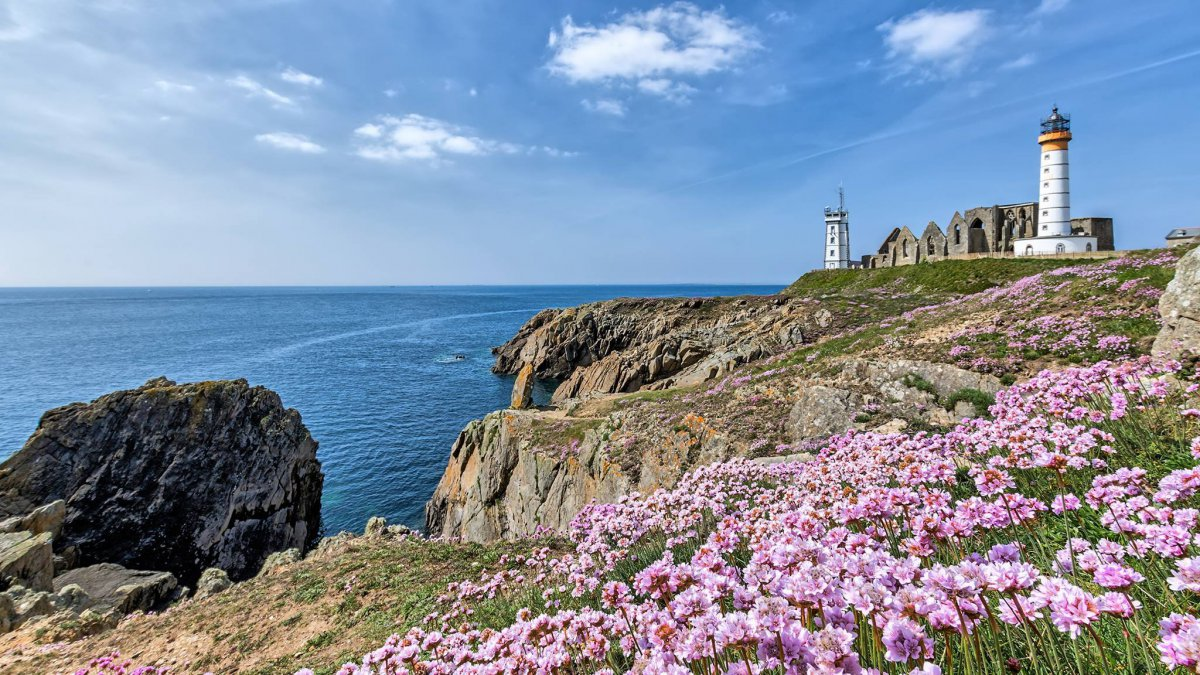
\includegraphics[width=0.7\linewidth]{Figures/saint_mathieu_avec_les_armeries_yann_quiviger-3215501}%
	\caption[Short caption goes to List of Figures]{This is a long caption; we can describe a lot of things here. For example, this photo is impressive. The shot was in Saint-Mathieu by Yann Quivig.}%
	\label{fig:test}
\end{figure}


% ------------------------------------------------------------------------------------------------------
\section{Another Section}\label{sec:another}
This is is a reference to the Chapter~\ref{chap:intro}.



\begin{table}[htb]
\caption{The effects of treatments X and Y on the four groups studied.}%
\label{tab:treatments}
\centering
\begin{tabular}{l l l}
\toprule
Groups & Treatment X & Treatment Y \\
\midrule
1 & 0.2 & 0.8\\
2 & 0.17 & 0.7\\
3 & 0.24 & 0.75\\
4 & 0.68 & 0.3\\
\bottomrule\\
\end{tabular}
\end{table}


\Blindtext%

\simplebox{%
\begin{otherlanguage}{french}
	\lipsum[4]%
\end{otherlanguage}
}

\lipsum[6]

\section{An extra section}
\Blindtext%
	
\Blindtext%

\begin{algorithm}
	\begin{algorithmic}[1]
		
		\STATE{\textbf{input:} $G$} \COMMENT{Graph}
		\STATE{\textbf{output:} $\mathcal{C}$} \COMMENT{Set  of all maximal cliques in G.}
		
		
		\STATE{adj $\leftarrow$ list all adjacent pairs in G}
		\STATE{Q $\leftarrow \emptyset$}   \COMMENT{Queue of candidates}
		
		\STATE{subg $\leftarrow$ list of all nodes in G}
		\STATE{cand $\leftarrow$ list of all nodes in G} \COMMENT{Candidates to be evaluated}
		
		\STATE{u $\leftarrow$ node in subg with highest cardinality}
		\STATE{ext\_u $\leftarrow$ list of nodes in cand except the set of adjacent of u}
		\STATE{stack $\leftarrow \emptyset$} \COMMENT{Execution stack}
		
		\WHILE{\TRUE{}}
		\IF{ext\_u $\ne \emptyset$}
		\STATE{q $\leftarrow$ POP(ext\_u)} \COMMENT{next node in the ext\_u list.}
		\STATE{cand $\leftarrow$ cand \arraybackslash {q}} \COMMENT{remove q node from cand.}
		\STATE{Q $\leftarrow$ PUSH(Q,q)} \COMMENT{Push q in the list Q.}
		\STATE{adj\_q $\leftarrow$ list of adjacent of q}
		\STATE{subg\_q $\leftarrow$ subgraph with all adjacents of q} 
		\IF{subg\_q $= \emptyset$}
		\STATE{$\mathcal{C}$ $\leftarrow$ Q}
		\ELSE{} 
		\STATE{cand\_q $\leftarrow$ set of nodes in cand adjacent to q}
		\IF{cand\_q $\ne \emptyset$}
		\STATE{stack $\leftarrow$ stack $\cup$ \{(subg, cand, ext\_u)\}}
		\STATE{Q $\leftarrow$ Q $\cup$ \{ \}}
		\STATE{subg $\leftarrow$ subg\_q}
		\STATE{cand $\leftarrow$ cand\_q}
		\STATE{u $\leftarrow$ node in subg with highest cardinality}
		\STATE{ext\_u $\leftarrow$ list of nodes in cand except the set of adjacent of u}
		\ENDIF{}
		\ENDIF{}
		
		\ELSE{}
		\STATE{POP(Q)}
		\STATE{subg, cand, ext\_u $\leftarrow$ POP(stack)}
		\ENDIF{}
		\ENDWHILE{}
		\RETURN{$\mathcal{C}$}
	\end{algorithmic}
	\caption{Output all maximal complete subgraphs.}\label{alg:fclique}	
\end{algorithm}

%\begin{algorithm}
%	\caption{test 2}
%\end{algorithm}
\subsection{Section 2}
\Blindtext%
\subsubsection{Section 2}
\Blindtext%
%\begin{algorithm}
%	\caption{test}
%\end{algorithm}
